\chapter{Implementation}
This chapter deals with the implementation details of the campus app. It starts by describing the process for the collection and processing of geodata and explains how the campus map and the navigation system are derived from it. It further showcases the procedure for gathering campus-relevant data from publicly available web sources and concludes with a description of the implementation process for the user interface, which finally merges the campus map, navigation and information layers.

\label{cha:implementation}
\section{Collection of geodata and POI}
Geodata refers to all data about geographic information. In the case of this thesis, it mainly consists of coordinate points, which describe certain campus-relevant entities, such as outlines of buildings, the street network, pathways, entrances as well as boundaries of green areas and water. Except for single-point usage, multiple coordinate points can be grouped into polygons, representing the closed outline of an entity and polylines, mainly used to describe lines, streets and paths. In addition to its coordinates, geodata also describes other attributes of an entity e.g., its name, altitude, width or height. This can be used for tasks like geocoding/reverse geocoding, display of information, 3d terrain generation or general data analysis.

\subsection{Overview of needed geodata}
Geodata is the building block for map generation and routing through a street network. The following list presents an overview of the geodata needed for this implementation:

\begin{itemize}
    \item Buildings: The outlines of buildings are polygons consisting of multiple coordinate points. Additionally to that, the height of each building is needed for appropriate 3D representation.
    \item Streets: Streets are represented by polylines and are (based on their importance, size and purpose) divided into three categories, namely main roads, small roads and pathways. This separation allows the different road types to be designed and displayed independently from each other. They can therefore vary in size, style and coloring when used in the campus map.
    \item Green areas: The outlines of green areas are retrieved in the polygon format.
    \item Water: The outlines of water (especially rivers) are also retrieved in the polygon format.
    \item Entrances to TU Berlin's buildings: To successfully connect TU Berlin's buildings to its underlying street network, entrances need to be defined. A single-point representation paired with an identifier for the buildings is used.
\end{itemize}

\subsection{Collection data from OSM via Overpass Turbo API}
OpenStreetMap (OSM) is a free mapping service, that allows its users to access, edit and download its available geodata. Its main querying language is Overpass Turbo which comes with a web interface for data mining and a respective web API \cite{openstreetmap_overpass_turbo}. This querying system is used to provide a starting point for the complete set of geodata needed for this thesis. The used bounding box for retrieval is (52.49993096650543, 13.307022255971093) for the south-west and (52.52269751545147, 13.341918533901309) for the north-east corner. The following table presents the queried data over all categories together with the node count (one node usually consists of a coordinate point), the type of retrieved data and the respective query.

\begin{table}[!ht]
	\small
	\centering
	\begin{tabular}{|l|l|l|l|}
		\hline
		Entities                & Type of geodata       & Number of queried nodes       & Overpass Turbo query \\
		\hline
        Buildings               & Polygons              & 1949                          & \ref{buildings} \\
		\hline
		Main roads              & Polylines             & 2036                          & \ref{main_roads} \\
		\hline
		Small roads             & Polylines             & 2578                          & \ref{small_roads} \\
		\hline
		Pathways and sidewalks  & Polylines             & 11757                         & \ref{pathways} \\
		\hline
        Green areas             & Polygons              & 5057                          & \ref{green_areas} \\
		\hline
        Water                   & Polygons              & 1651                          & \ref{water} \\
		\hline
        Entrances               & Single points         & 1758                          & \ref{entrances} \\
		\hline
	\end{tabular}
	\caption{Overview of queried geodata}
\end{table}

This results in a total of 26786 queried nodes. Each category is further exported as a separate geojson file, containing the relations between individual points (polygon, polyline, single node) as well as other OSM attributes (e.g., the names of buildings and streets, the height of buildings, etc.).

\subsection{Correction of OSM data for map generation in QGIS}
Since the queried data contains several imperfections that are not desirable for map generation, all geojson files are imported into QGIS for cleanup. QGIS is an open-source geographic information system, that provides a convenient visual user interface for editing geodata. The following images present a visual reference for the changes performed to the data (note, that all street data is represented in one image for simplicity and that water data does not need cleanup and is therefore not present).

\begin{figure}[H]
	\centering
	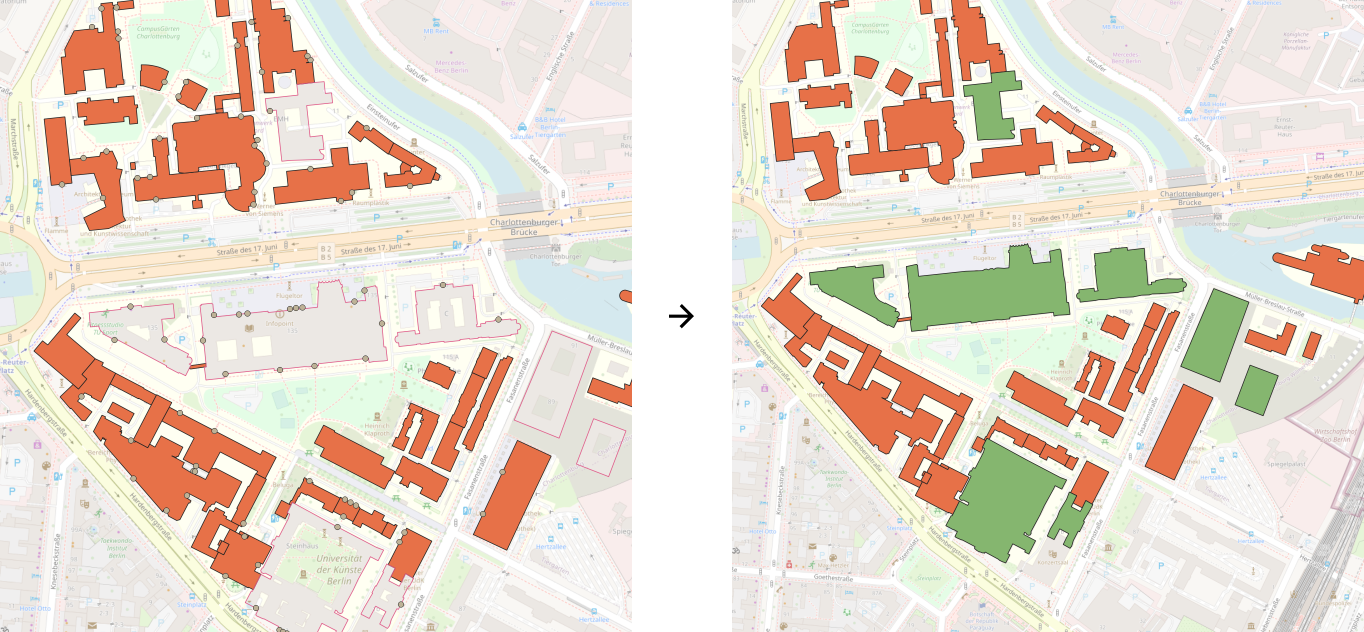
\includegraphics[width=0.65\textwidth]{images/preparing_buildings.png}\\
	\caption{Correction of TU Berlin's building data}
\end{figure}

\begin{figure}[H]
	\centering
	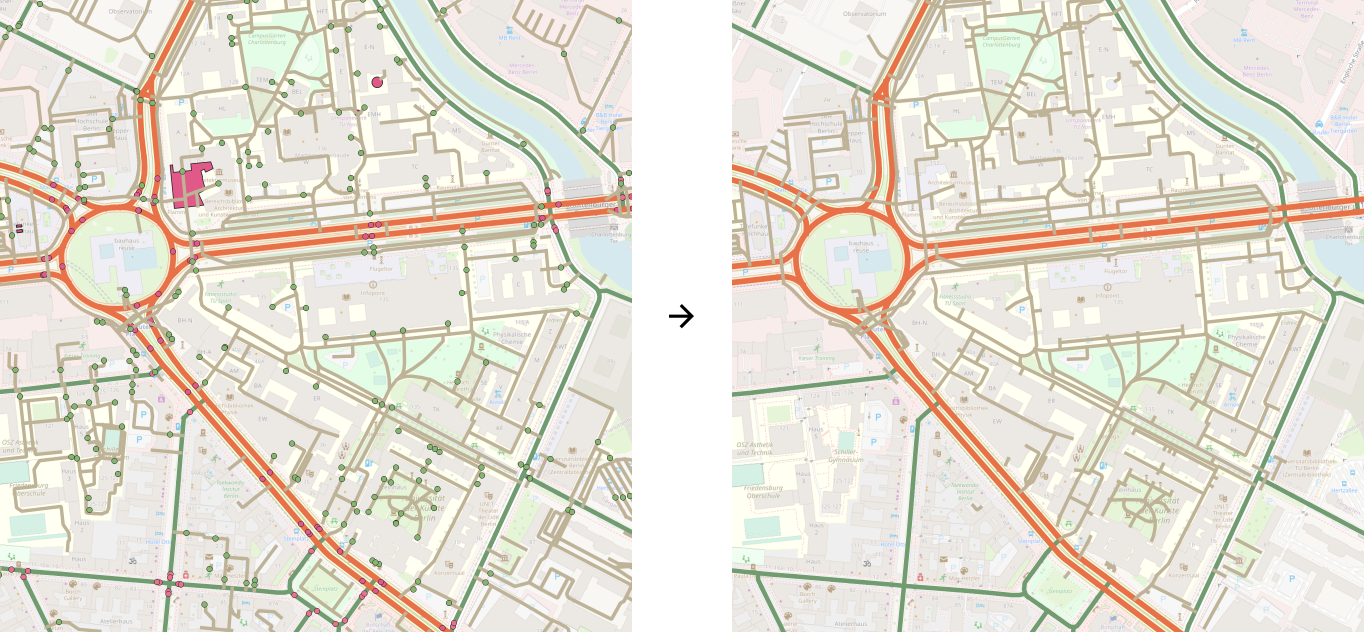
\includegraphics[width=0.65\textwidth]{images/preparing_streets.png}\\
	\caption{Correction of TU Berlin's street network data}
\end{figure}

\begin{figure}[H]
	\centering
	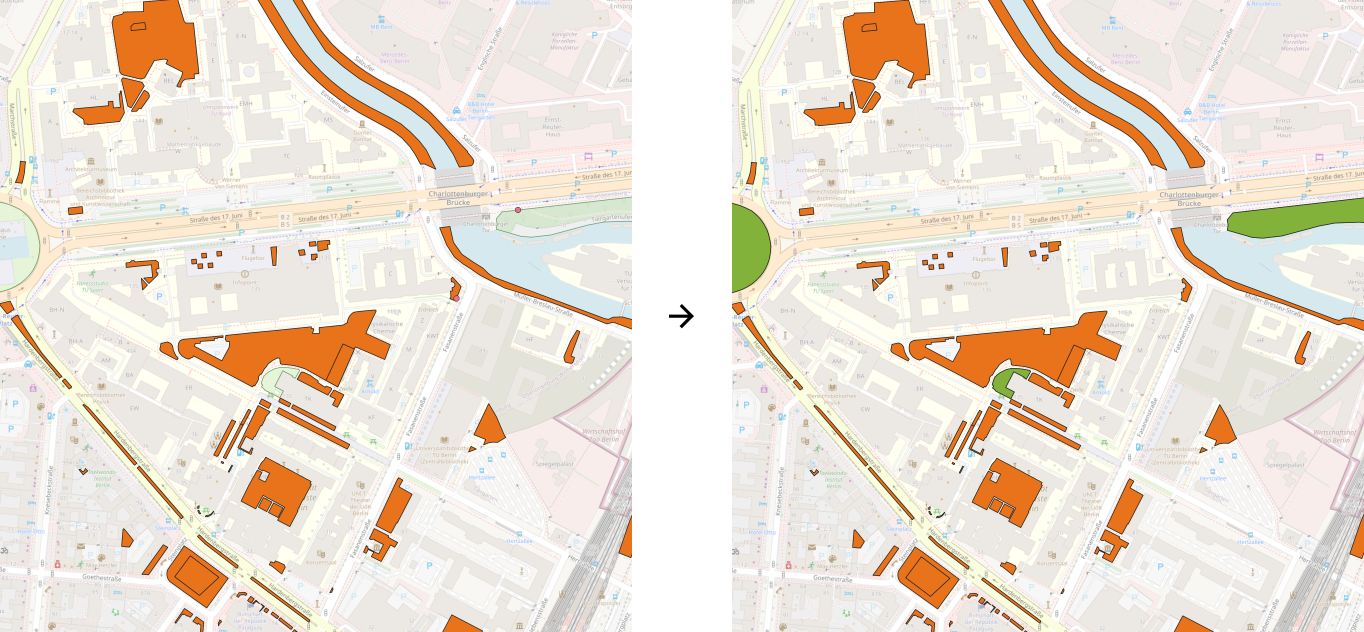
\includegraphics[width=0.65\textwidth]{images/preparing_green_areas.png}\\
	\caption{Correction of TU Berlin's green area data}
\end{figure}

\begin{figure}[H]
	\centering
	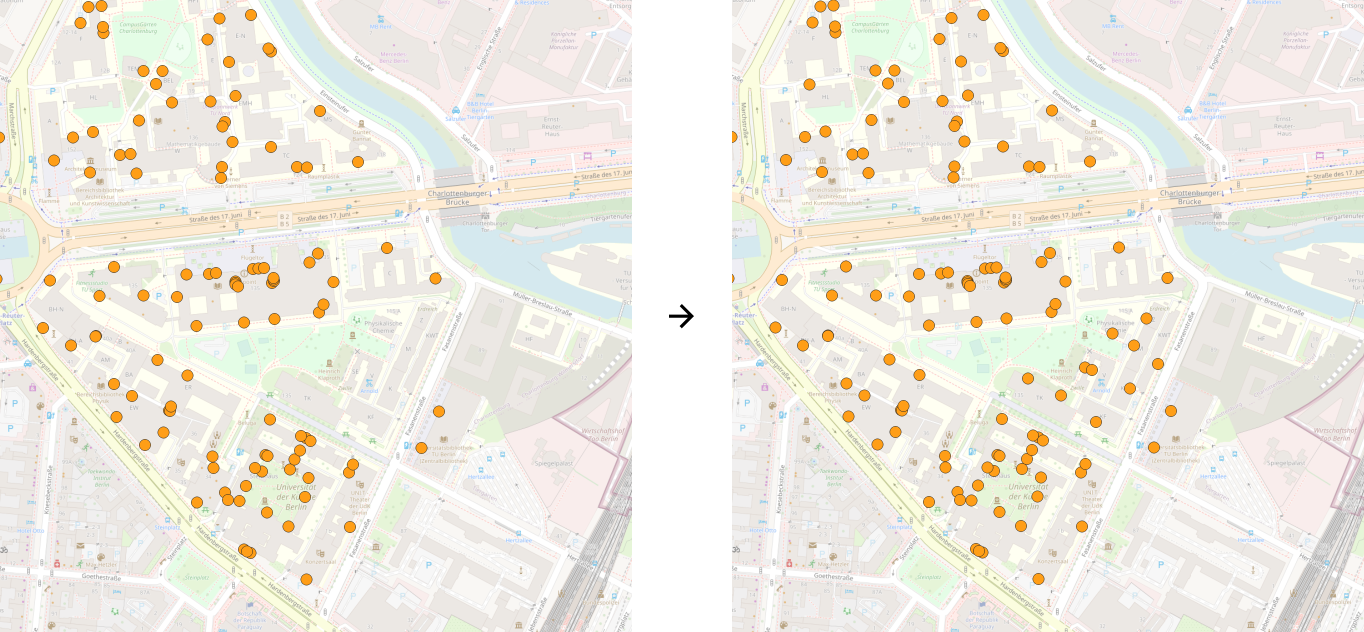
\includegraphics[width=0.65\textwidth]{images/preparing_entrances.png}\\
	\caption{Correction of TU Berlin's entrance data}
\end{figure}

The main problem that gets corrected consists of wrong geometry types in the data. Since is desirable that every dataset only contains one kind of geometry (e.g., the data for the buildings should only contain polygon outlines, the street data should only contain polylines, etc.), all wrong geometry types in a dataset are either deleted (e.g., single points in the street or building data) or reshaped to match the expected geometry type (e.g., polylines representing the outline of a building/green area are converted into polygons).

Missing entities (e.g., certain entrances to buildings) are furthermore added and information not related to the campus (mainly data from the street network) is removed.

\section{Generation of digital campus map}
Das ist ein Test.

\subsection{Data import and conversion in Unity}
\subsection{Mesh generation for streets, green areas, water and 3d buildings}
\subsection{Map design}
\subsection{Integration into the Flutter app}

\section{Navigation system development}
\subsection{Representation of geodata for navigation}
\subsection{Manual generation of TU Berlin's street network}
\subsection{Routing across the campus}
\subsection{Time estimation for routes}
\subsection{Embedding the current user location via GPS}

\section{Interactive information layer development}
\subsection{Collection of campus relevant information from the web}
\subsection{Processing of information and internal representation}

\section{User interface development}
\subsection{Navigation system}
\subsection{Information layer}
\subsection{Enhancing the user experience with additional screens and features}